% Section 1, Introduction.
\section{Introduction}
\label{sec:intro}

Frontier-model agents now resolve real repository issues, from locating
bugs to generating patches~\citep{swebench}, but each solve carries a
real per-task price.  Strong open-weights models cost a fraction yet
close fewer tasks.  Any team deploying an issue-solving system therefore
faces a standing choice between the expensive best model and cheaper
alternatives.  Existing LLM routers~\citep{routellm,frugalgpt} make
that choice from the task text alone, before anything has engaged with
the actual repository.

Replaying learned routers over the public per-task results of three SWE
benchmarks reveals that solve sets are largely nested: models that solve
more tasks nearly always subsume the solve sets of weaker ones, and no
router reliably improves on always selecting the strongest
model~(\S\ref{sec:problem}).  Routing for accuracy therefore offers
little headroom.  Routing for \emph{cost}, by contrast, only requires
predicting when a cheaper model will suffice.

\begin{figure}[!tbp]
\centering
% ===========================================================================
% fig-cost-solve.tex — cost-per-solve vs solve-rate scatter, with the
% kimi<->opus blind-mixing line.
% BODY ONLY (tikzpicture). Wrapper/caption/label live in the section file.
% Requires % ===========================================================================
% fig-style.tex — shared colour / marker scheme for EVERY main-paper figure.
% \input this ONCE from the preamble of main.tex (after tikz + pgfplots).
%
% House rule: the palette is defined here and nowhere else. Each series also
% gets a distinct marker AND line style so the figures survive grayscale
% printing.
%
%   \sysname / deployed .. cSys   (blue!70!black)    mark *
%   opus / claude ........ cOpus  (red!70!black)     mark square*
%   gpt .................. cGpt   (teal!70!black)    mark triangle*
%   kimi ................. cKimi  (violet!70!black)  mark diamond*
%   flash ................ cFlash (orange!70!black)  mark pentagon*
%   greedy / baseline .... cBase  (gray)             mark o
% ===========================================================================
% The pipeline diagram needs the calc library for coordinate arithmetic; the
% rest of the libraries are already loaded in main.tex's preamble.
\usetikzlibrary{calc}
% Hatching, so bar charts stay readable in grayscale.
\usetikzlibrary{patterns}

\colorlet{cSys}{blue!70!black}
\colorlet{cOpus}{red!70!black}
\colorlet{cGpt}{teal!70!black}
\colorlet{cKimi}{violet!70!black}
\colorlet{cFlash}{orange!70!black}
\colorlet{cBase}{gray}

% Common axis furniture: footnotesize ticks/legend, small titles, framed
% legend in gray!50, light horizontal grid.
\pgfplotsset{
  paperaxis/.style={
    width=0.80\linewidth,
    height=5.2cm,
    tick label style={font=\footnotesize},
    label style={font=\footnotesize},
    title style={font=\small},
    legend style={font=\footnotesize, draw=gray!50, fill=white,
                  fill opacity=0.9, text opacity=1, rounded corners=1pt},
    every axis plot/.append style={line width=0.7pt},
    grid style={gray!25, line width=0.3pt},
    axis line style={gray!60},
    tick style={gray!60},
  },
  papermark/.style={mark size=2.6pt},
}
 in the preamble.
% Provenance: data/receipts/outcomes_per_task.json and
%             data/receipts/routing_scenarios.json.
%
% Design notes:
%   - The router point and the no-router ablation differ by $0.003 per solve,
%     under 1.5pt on this log axis, so they share ONE composite glyph (open
%     cKimi diamond for the ablation, smaller filled cSys disc drawn last
%     inside it) with one colour-keyed callout and one leader; two markers
%     would misstate the resolution of the figure.
%   - The mixing reference is convex in LINEAR cost, so it is sampled as the
%     true mixture and renders as a curve on a log-x axis.
% ===========================================================================
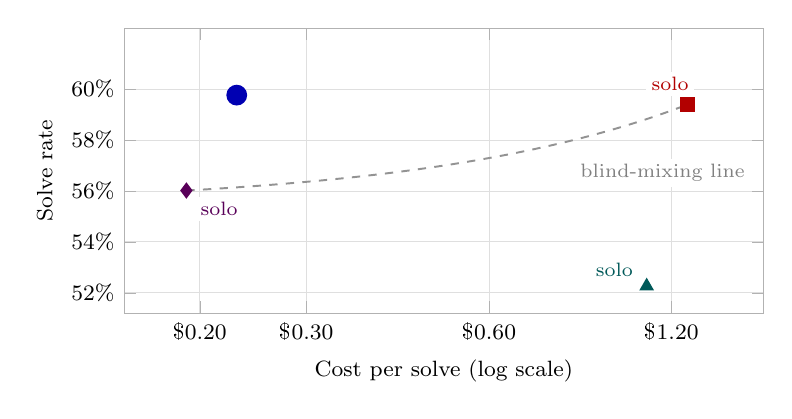
\begin{tikzpicture}
\begin{axis}[
  paperaxis,
  xmode=log,
  log basis x=10,
  xmin=0.150, xmax=1.70,
  ymin=51.2, ymax=62.4,
  xtick={0.2,0.3,0.6,1.2},
  xticklabels={\$0.20,\$0.30,\$0.60,\$1.20},
  log ticks with fixed point,
  xminorticks=false,
  ytick={52,54,56,58,60},
  yticklabel={\pgfmathprintnumber{\tick}\%},
  xlabel={Cost per solve (log scale)},
  ylabel={Solve rate},
  ymajorgrids=true,
  xmajorgrids=true,
]

% --- blind-mixing locus: kimi -> opus (reference, deliberately subdued) --
% Solve rate is affine in LINEAR cost, so on a log-x axis this is a CURVE,
% not a straight segment; drawing it straight would overstate the baseline.
% Sampled densely; the endpoints are exactly the two solo points.
\addplot[dashed, line width=0.7pt, color=cBase!85, mark=none, forget plot,
         domain=0.190:1.274, samples=120, smooth]
  {56.02 + (x-0.190)*(59.40-56.02)/(1.274-0.190)};

% --- solo anchors (context) ---------------------------------------------
\addplot[only marks, mark size=2.4pt, color=cOpus, mark=square*, forget plot]
  coordinates {(1.274,59.40)};
\addplot[only marks, mark size=2.4pt, color=cKimi, mark=diamond*, forget plot]
  coordinates {(0.190,56.02)};
\addplot[only marks, mark size=2.4pt, color=cGpt, mark=triangle*, forget plot]
  coordinates {(1.091,52.26)};

% --- \sysname (protagonist): larger mark, drawn last, on top ------------
% The no-router ablation is deliberately NOT plotted here; it lives in the
% main results table. The figure carries the headline only.
\addplot[only marks, mark size=3.3pt, color=cSys, mark=*,
         mark options={fill=cSys, draw=cSys, line width=0.9pt}, forget plot]
  coordinates {(0.230,59.77)};
\node[font=\scriptsize, color=cSys, anchor=south, inner sep=1.5pt, fill=white]
  at (axis cs:0.230,60.05) {\textbf{\sysname}};

% --- inline labels ------------------------------------------------------
% Placement rule: each label is anchored so its box lies in a quadrant no
% marker, no grid tick and no segment of the dashed line passes through.
\node[font=\scriptsize, color=cOpus, anchor=south east, inner sep=2pt, fill=white]
  at (axis cs:1.310,59.70) {\fxopusS solo};
\node[font=\scriptsize, color=cKimi, anchor=north west, inner sep=2pt, fill=white]
  at (axis cs:0.196,55.80) {\fxkimiS solo};
\node[font=\scriptsize, color=cGpt, anchor=south east, inner sep=2pt, fill=white]
  at (axis cs:1.060,52.40) {\fxgptS solo};
\node[font=\scriptsize, color=cBase, anchor=north east, inner sep=2pt, fill=white]
  at (axis cs:1.620,57.30) {blind-mixing line};

\end{axis}
\end{tikzpicture}

\caption{\textbf{Cost per solve versus solve rate on SWE-bench Pro
(Python-266).}  The dashed curve is the blind-mixing line (random
cost-blind mix of \fxkimi and \fxopus).  \sysname matches \fxopus at
about a fifth of its cost per solve, well above the line.  The system
point is all-in; solo points are fixer API only.  The $x$-axis is
logarithmic.}
\label{fig:cost-solve}
\end{figure}

\sysname routes \emph{after} scouting, a pattern we call
\emph{scrouting}.  A 7B searcher,
\modelname, first explores the repository and produces a structured
handoff: a list of implicated files, diagnostic notes, and a candidate
reproduction test.  These claims pass through a sandbox verification
step, and claims that do not check out are stripped before a downstream
model ever sees them.
A r\'esum\'e router then selects among four frontier fixers using the
task text together with the searcher's own hidden states; adding a new
fixer requires no retraining.

Figure~\ref{fig:cost-solve} compares \sysname to solo frontier models on
SWE-bench Pro's full Python slice~\citep{swebenchpro} (266 tasks),
matching the benchmark's official capped budget tier exactly.  \sysname
matches the best single frontier model's solve rate, resolving 159 of
266 tasks versus 158, at \$0.230 total cost per solve compared to
\$1.274: about a fifth.  The configuration sits above the blind-mixing
line (the accuracy/cost segment any random split of traffic between a
cheap and a strong model would achieve).  The searcher's contribution to
system cost is negligible: \modelname's entire GPU bill for the
evaluation was \$1.13.

A paired calibration study on 100 fresh tasks points to why this cost
reduction holds: the handoff appears to redistribute rather than add
solving ability, lifting the three cheaper fixers while slightly hurting
the strongest, and the
searcher's hidden states improve cost routing where the handoff's own
text does not~(\S\ref{sec:calibration}).

We make five contributions:
\begin{itemize}
  \item An engage-then-route architecture with a trained searcher whose
    verified handoff is consumed by the chosen fixer.
  \item A zero-cost replay audit of published per-task outcomes on three
    SWE benchmarks showing that solve sets are largely nested and that no
    learned router reliably beats always calling the strongest model,
    which motivates routing for cost rather than accuracy.
  \item Routing features drawn from the searcher's hidden states, with a
    r\'esum\'e-based $N$-way pool where adding a new fixer requires no
    retraining.
  \item A matched-protocol evaluation on SWE-bench Pro's Python census
    showing frontier-matching accuracy at about a fifth of the total
    cost per solve.
  \item A paired calibration study measuring the handoff's
    redistribution pattern and the router's feature design space, plus a
    verification gate that strips the searcher's false reproduction
    claims.
\end{itemize}
